\begin{tikzpicture}
\node[inner sep=0,anchor=south west] (im) at (0,0) {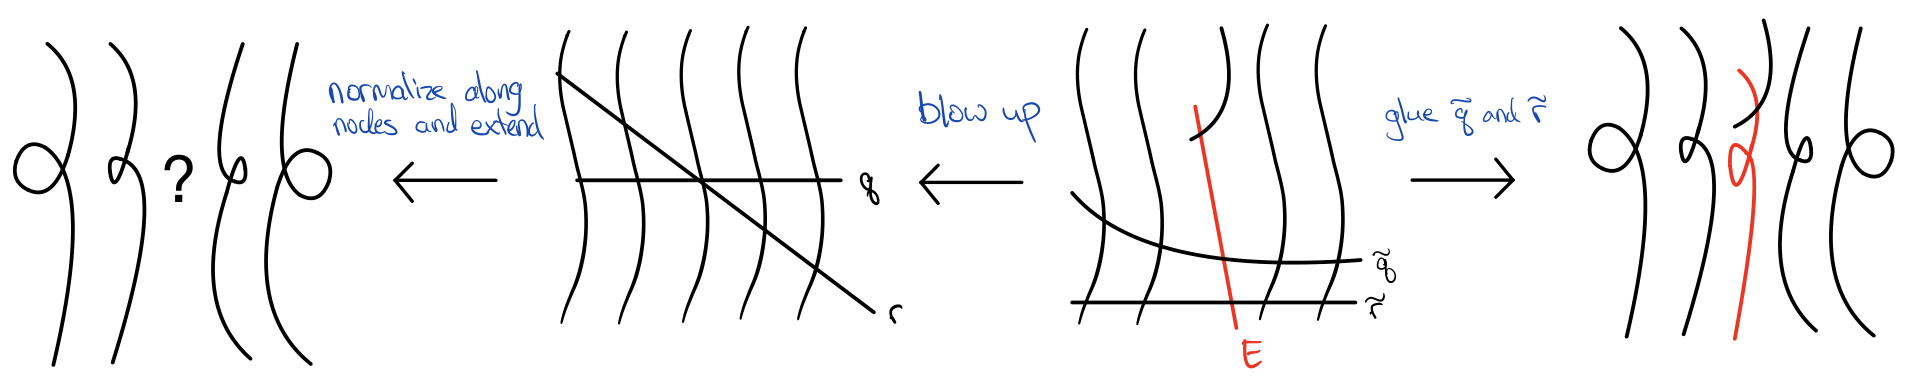
\includegraphics[width=.86\textwidth]{figures/reduction-step1.png}};
\begin{scope}[x={(im.south east)},y={(im.north west)}]
\fill[white] (0.17,0.62) rectangle (0.29,0.84);
\fill[white] (0.47,0.65) rectangle (0.56,0.8);
\fill[white] (0.72,0.64) rectangle (0.83,0.8);
\node[fill=white,inner sep=1pt,font=\scriptsize,text=blue] at (0.23,0.75) {沿结点正规化};
\node[fill=white,inner sep=1pt,font=\scriptsize,text=blue] at (0.23,0.64) {并延拓};
\node[fill=white,inner sep=1pt,font=\scriptsize,text=blue] at (0.514,0.7) {爆破};
\node[fill=white,inner sep=1pt,font=\scriptsize,text=blue] at (0.774,0.7) {粘合 $\widetilde q,\widetilde r$};
\end{scope}\end{tikzpicture}
